\documentclass{article}
\usepackage{graphicx}
\usepackage{hyperref}

\begin{document}

\title{The HypeDyn Hypertext Fiction Editor\\Tutorial 1: Nodes, Links and Rules}
% \author{Alex Mitchell}
\date{}

\onecolumn
\maketitle

\tableofcontents


\section{Introduction}
In this tutorial, we will build a basic interactive story in the HypeDyn
hypertext fiction editor. HypeDyn is a tool which lets you create ``hypertext'',
a form of writing which usually consists of:

\begin{itemize}
  \item A collection of text fragments or ``nodes'', containing some text, which
  are normally displayed one at a time in a hypertext reader;
  \item ``links'' between these nodes, which provide a connection from one node,
  or more commonly from a section of text in one node, to another node. A reader
  is usually able to ``follow'' a link to its destination node by, for example,
  clicking on the link; 
  \item ``rules'' which can be attached to a link, which contain
  a set of conditions, and a set of actions, such as following a link, which
  are performed if the rule's conditions are satisfied.
\end{itemize}

In this tutorial, we will be creating a simple hypertext \textit{fiction}.
Hypertext fiction usually consists of a story told in hypertext. Most well-known
examples of hypertext fiction let the reader explore through a set of text
fragments, encouraging them to discover different paths through the story. These
alternate paths sometimes uncover new information which the reader didn't
previously know, thereby altering their perception of the story.

Our example, ``Little Red Riding Hood'', involves the reader exploring several
paths through a story. The main path tells a simplified version of the
traditional folk tale, about a little girl with a red hood who meets a wolf on
the way to visit her Grandmother. An addtional side path, which can only be accessed once
the reader has visited the last node in the main path, reveals some additional
background information about Red's hood.


\begin{figure}[ht]
  \centering
  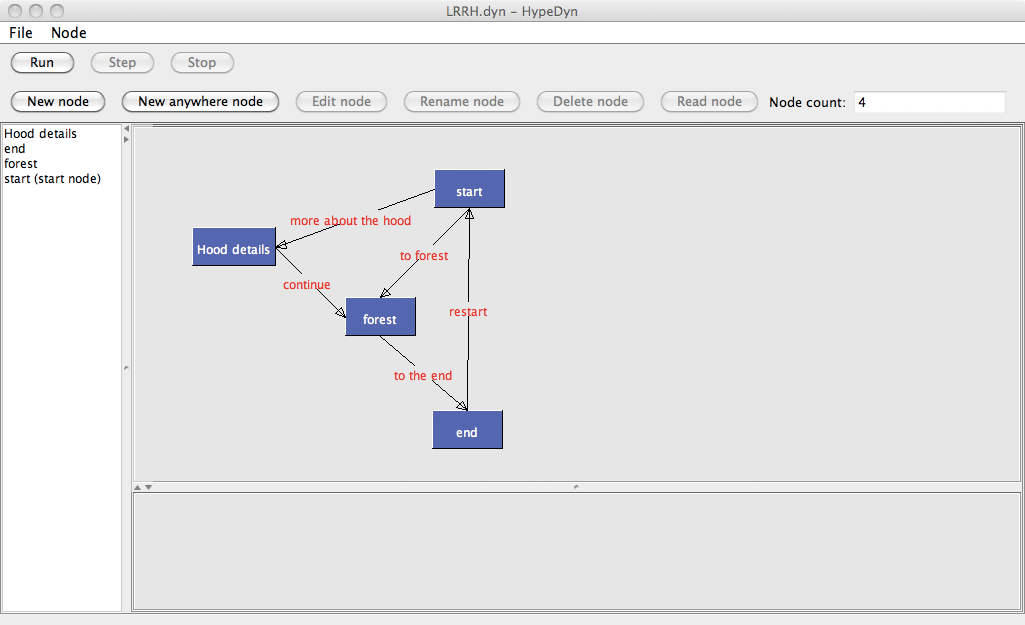
\includegraphics[width=10cm]{images/hypedyn-tutorial-1-figure-1}
  \caption{\textit{The completed ``Little Red Riding Hood'' story.}}
  \label{fig:tut1:completed_story}
\end{figure} 

The nodes and links in the final story are shown in Figure
\ref{fig:tut1:completed_story}. Although this is a very simple story, it will involve
most of the basic functionality of HypeDyn.

\textit{Note:  HypeDyn is a work-in-progress, so there are some features that are still
not completed, and there may be bugs. If you encounter any errors, please
report them as bugs on our Launchpad site: \url{https://launchpad.net/hypedyn}.}

\section{Getting started}

First, open HypeDyn by double-clicking on the file \textbf{HypeDyn.exe} (in
Windows) or \textbf{HypeDyn.app} (in MacOS).

Save your file by choosing Save from the File menu. Make sure that you give the
file a \textbf{.dyn} extension.

\section{Creating a text node}

The first thing we need to do is to start creating some text nodes. We'll begin
by creating the starting node, which represents the first fragment in the story.
In this node, we will introduce the main character, Red, and the initial action of
the story, the fact that she is walking through the forest.
 
\begin{figure}[ht]
  \centering
  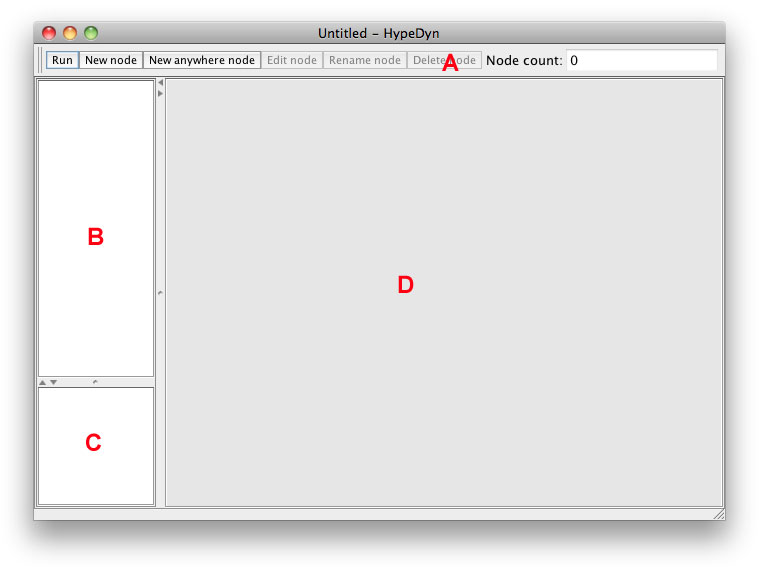
\includegraphics[width=10cm]{images/hypedyn-tutorial-1-figure-2}
  \caption{\textit{The main HypeDyn interface.}}
  \label{fig:tut1:hypedyn}
\end{figure} 

The main HypeDyn interface consists of the Toolbar (A), the Node list (B), the
Fact list (C), and the Map view (D), as shown in Figure \ref{fig:tut1:hypedyn}.
The Toolbar contains the functions that we will use to create and edit our text
nodes. The Node list contains a list of the nodes in your story. The Fact list
contains a list of the facts in your story.
The Map view displays the nodes and links. The Map view contains two different
types of nodes: regular nodes and anywhere nodes. We will not be using facts or
anywhere nodes in this tutorial.

\begin{enumerate}
  \item To create a new text node, click on the New node button. A new text node
  will be created, and you will be asked to give it a title. Name the new text
  node ``Start'', and click Ok, as shown in Figure \ref{fig:tut1:new_node}.
\end{enumerate}

 
\begin{figure}[ht]
  \centering
  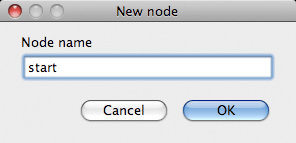
\includegraphics[width=5cm]{images/hypedyn-tutorial-1-figure-3}
  \caption{\textit{Creating a new text node.}}
  \label{fig:tut1:new_node}
\end{figure} 

Text nodes are the basic building blocks of hypertexts created with HypeDyn.
Each text node has: 
\begin{enumerate}
  \item A title to identify the node
  \item Some text content.
\end{enumerate}

Once you've created a text node, you should see the node represented in both the
node list and the Map view (see Figure \ref{fig:tut1:first_node}). You can select the
node by clicking on its title in the node list.
 
\begin{figure}[ht]
  \centering 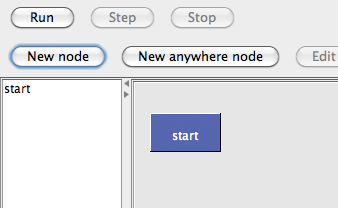
\includegraphics[width=8cm]{images/hypedyn-tutorial-1-figure-4}
  \caption{\textit{Our first node showing in the Node list and Map view.}}
  \label{fig:tut1:first_node}
\end{figure} 

You can also drag the node around in the Map view by selecting the node and then
dragging it. Once we have created several nodes and links between them, it can
be useful to position them in the Map view so that we can easily see the
relationship between them. However, the position of the nodes in the Map view
does not change their behaviour in any way.

\section{Adding text to a node}

Now that we have our first text node, we need to go in and enter some text.

\begin{enumerate}
  \item Choose the title of our node, start, in the node list, and then click
  on the Edit node button in the Toolbar. This will open the editing view for
  the node, as shown in Figure \ref{fig:tut1:edit_node}. 
  
\begin{figure}[ht]
  \centering
  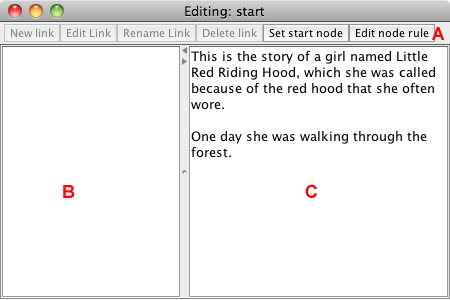
\includegraphics[width=9cm]{images/hypedyn-tutorial-1-figure-5}
  \caption{\textit{The editing view of a text node.}}
  \label{fig:tut1:edit_node}
\end{figure} 

The Editing view lets you enter the text for a node. It also lets you add, edit
and delete links. The Editing view consists of the Toolbar (A), the Link list (B),
and the Content editor (C).

Note that the name of the node that you are currently editing is shown in the
title bar of the Editing view.

\item Now enter the text for the first fragment of our story in the Content
editor:

\textit{This is the story of a girl named Little Red Riding Hood, which she was
called because of the red hood that she often wore.}

\textit{One day she was walking through the forest.}

\item We want this node to be the start of our story, so click on the Set start
node button to set this node as the start node. Every story must have a start
node. The start node is indicated by the words ``(start node)'' shown after the
node name in both the Node list and the Map view.
\item Once you've finished entering this text, close the editing view by
clicking on the close button. This will take you back to the Map view.
\end{enumerate}

\section{Creating links between nodes}

We will now create several other nodes, to represent other fragments of our
hypertext story, and we'll create links between them.

\subsection{Creating the other nodes}

\begin{enumerate}
  \item Create another text node, and name it ``forest''.
  \item Enter the following text in the node:

\textit{In the forest, Red came across a young man with a nasty smile.}

\textit{``Where are you going, little girl?'' he asked.}

\textit{``I'm off to see my sick granny,'' she said.}

\textit{Well, you can probably guess what happened next.}

This node represents the main conflict of the story.

\item Create a third node, and name it ``end''.
\item Enter the following text in the node:

\textit{*** The End ***}

\textit{back to start}

This node represents the end of our story.
\end{enumerate}

You should have three nodes: ``start'', ``forest'', and ``end'', as in
Figure \ref{fig:tut1:three_nodes}.

 
\begin{figure}[ht]
  \centering
  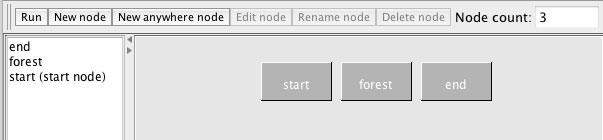
\includegraphics[width=12cm]{images/hypedyn-tutorial-1-figure-6}
  \caption{\textit{Three text nodes.}}
  \label{fig:tut1:three_nodes}
\end{figure} 

\subsection{Creating a link}

Now we want the user to be able to move from one text node to another, as they
make decisions about how to read the story. To do this, we need to create links
between the nodes.

Links in HypeDyn can be attached to a specific piece of text. When the user
clicks on a link, one or more rules are triggered. These rules are where the
author can specify what will happen when the link is clicked. For example, in our
story, we want the user to be able to click on ``forest'' in the ``start'' node
to jump to the ``forest'' node. This lets the user progress through the main
story path.

\begin{enumerate}
  \item Select the ``start'' node in the Node list, and then click on the Edit
  node button.
  \item Now select the word ``forest''. We'll attach our link here.
  \item Click on the New link button in the Editing view. A New link dialogue
  box will appear, as shown in Figure \ref{fig:tut1:create_link}.

\begin{figure}[ht]
  \centering
  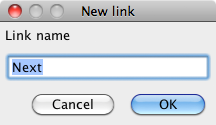
\includegraphics[width=4cm]{images/hypedyn-tutorial-1-figure-7}
  \caption{\textit{Creating a link.}}
  \label{fig:tut1:create_link}
\end{figure} 

\item Give the link a name, such as ``Next'', and click OK. \item You will now
see the ``Edit link'' dialogue (see Figure \ref{fig:tut1:edit_link_1}). This is where
we can specify the rules for the link.

The ``Edit link'' dialogue consists of a list of rules, each of which will be
triggered when the user clicks on the link. For now, we will create a single
rule, which will jump the story to the ``forest'' node.

\begin{figure}[ht]
  \centering
  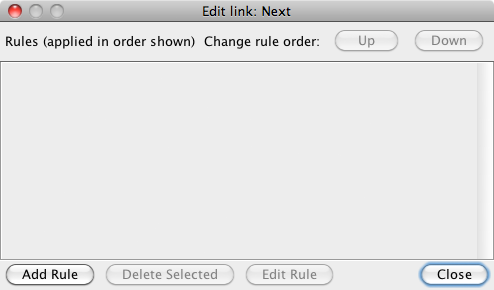
\includegraphics[width=9cm]{images/hypedyn-tutorial-1-figure-8}
  \caption{\textit{The ``Edit link'' dialogue.}}
  \label{fig:tut1:edit_link_1}
\end{figure} 

\item Click on the Add Rule button at the bottom left of the ``Edit link''
dialogue. A rule, named ``new rule'', will be added to the list of rules (see
Figure \ref{fig:tut1:new_rule}).

\begin{figure}[ht]
  \centering
  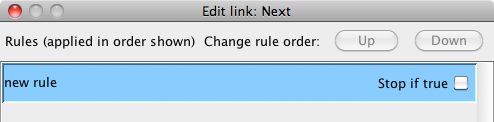
\includegraphics[width=9cm]{images/hypedyn-tutorial-1-figure-8b}
  \caption{\textit{Adding a rule to the ``Edit link'' dialogue.}}
  \label{fig:tut1:new_rule}
\end{figure} 

\item The new rule is initially selected. Click on the Edit rule button to edit
the rule. You will now see the ``Edit rule'' dialogue (see Figure
\ref{fig:tut1:edit_rule}).

\begin{figure}[ht]
  \centering
  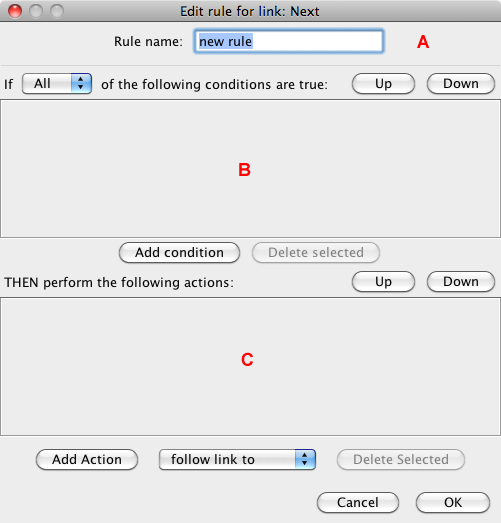
\includegraphics[width=9cm]{images/hypedyn-tutorial-1-figure-8c}
  \caption{\textit{The ``Edit rule'' dialogue.}}
  \label{fig:tut1:edit_rule}
\end{figure} 

The ``Edit rule'' dialogue consists of three sections: the \textit{rule name} (A)
which allows you to edit the name of the rule, the \textit{conditions} (B)
listing a series of conditions which specify when the rule can be triggered, and
the \textit{actions} section (C) which is the set of actions that are performed
when the conditions are satisfied. We will return to the conditions below.

\item First edit the name of the rule, changing it to ``Next''. This is the
label which will be placed on the link when it is displayed in the Map view.

\item Next, create the action. Select ``follow link to'' in the pull-down menu
beside the ``Add Action'' button, and click on the ``Add Action'' button. An
action will be added to the action list.

\item In the new action, use the pull-down menu to choose the ``forest'' node.
This will create a link from the text ``forest'' in the ``start'' node to the
``forest'' text node (see Figure \ref{fig:tut1:create_action}).

\begin{figure}[ht]
  \centering
  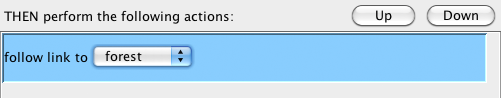
\includegraphics[width=9cm]{images/hypedyn-tutorial-1-figure-8d}
  \caption{\textit{Creating the rule to follow a link from ``start'' to
  ``forest''.}}
  \label{fig:tut1:create_action}
\end{figure} 

\item Now click OK in the ``Edit rule'' dialogue, and ``Close'' in the ``Edit
link'' dialogue.
\end{enumerate}

We have now created a link from the ``start'' node to the ``forest''. You
should be able to see this link in the Link list at the top of the Editing
view, and in the Map view, as shown in Figure \ref{fig:tut1:new_link_mapview}.
  
\begin{figure}[ht]
  \centering
  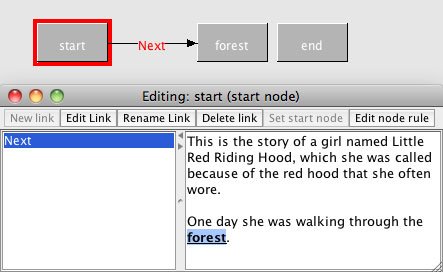
\includegraphics[width=10cm]{images/hypedyn-tutorial-1-figure-9}
  \caption{\textit{The link from the ``start'' to the ``forest''.}}
  \label{fig:tut1:new_link_mapview}
\end{figure} 

Notice that links show up as bold, underlined text in the content of the text node.

\subsection{Testing the link}

Now that we've created the link, we need to test that it works.

To switch from editing to reading the text nodes, we need to use the Run button
in the Toolbar in the Map view.

\begin{enumerate}
  \item Close the ``start'' node if its still open.
  \item Now click on the Run button. HypeDyn will open the Reader in a web
  browser window, showing the contents of the text node. You are now
  ``reading'' the story, instead of editing it, as shown in Figure
  \ref{fig:tut1:reading}.

\begin{figure}[ht]
  \centering
  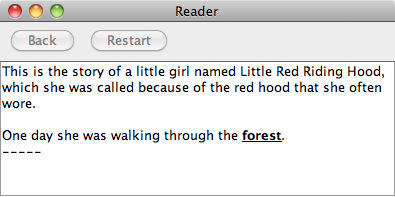
\includegraphics[width=9cm]{images/hypedyn-tutorial-1-figure-10}
  \caption{\textit{Reading a text node.}}
  \label{fig:tut1:reading}
\end{figure} 

In the Reader, you can click on links, and you'll be taken to the text node
that the link leads to.

\item Click on the word ``forest'' to follow the link.
\item The Reader will change to show the contents of the ``forest'' node.
\end{enumerate}

You can finish reading the story by closing the Reader window.

% this should be fixed now
% \textit{Note: For now, be careful not to give two links the same names, even if they
% are in different nodes. There used to be a bug in HypeDyn which makes it
% difficult to delete links with the same name. I think this has been fixed, but
% its better to be safe than sorry\ldots}

\subsection{Creating more links}

Now that we have one link from the ``start'' to the ``forest'', we should link
in our third node, ``end''. This will allow the user to move forward along the
main story path from the ``forest'' node to the ``end'' node, the end of the story.

\begin{enumerate}
\item Open the ``forest'' text node.
\item Select the word ``next''.
\item Click on the New link button.
\item Name this link ``to the end''.
\item Create a rule, and edit the rule. Name the rule ``to the end''.
\item Now add a ``follow link to'' action, and select the ``end'' node in the
pull-down menu.
\item Click on the Ok button, and close the link editor.

You now have a link to the ``end'' text node. Test this out by running
the story. You should be able to click on the ``forest'' link to move to the
``forest'' node, and then click on ``next'' to move to the ``end'' node.
 
\begin{figure}[ht]
  \centering
  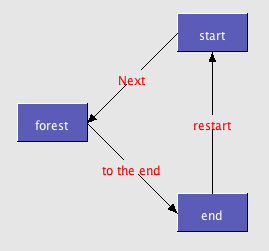
\includegraphics[width=6cm]{images/hypedyn-tutorial-1-figure-11}
  \caption{\textit{Three nodes with a loop back to the start.}}
  \label{fig:tut1:three_nodes_and_links}
\end{figure} 

Now we'll create one more link, this time from the ``end'' node back to the
``start'', so that the reader can re-read our story if they want.

\item Open the ``end'' node.
\item Select the words ``back to start''.
\item Click on the New link button.
\item Name this link ``restart''.
\item Create a rule, and edit the rule. Name the rule ``restart''.
\item Now add a ``follow link to'' action, and select the ``start'' node from
the pull-down menu.
\item Click on the Ok button, and close the link editor.
\end{enumerate}

We now have a loop back to the start. At this point, your Map view should look
as shown in Figure \ref{fig:tut1:three_nodes_and_links}.

\section{Creating rules with conditions}

The next thing we want to do is create a rule with conditions. This is a rule
that can only be triggered if a certain condition, such as the user having
visited a specific node, is satisfied.

We will create a node, named ``Hood details'', which can be reached after the
reader has read the entire story. This node will reveal additional information
that will (hopefully) change the reader's experience of the story, as the reader
will now know that there is something unusual, and perhaps slightly sinister,
about Red's hood.

To do this, we will use a feature in HypeDyn called a ``condition'' to only allow
the reader to see the ``Hood details'' node after they have seen the ``end''
node. This allows us, as the author of the story, to ensure that the reader has
gone through the main story path at least once. We want the reader to experience
the original story before seeing the new information, so that the new information
can more effectively impact their previous mental model of the events of the
story.

\subsection{Creating the node}

First we'll create a new node to contain the information about the hood.

\begin{enumerate}
  \item Create a new node, and name it ``Hood details''.
  \item Enter the following text in the text node:

\textit{Her hood was a magic garment, given to her by her grandmother.
It could kill anyone who tried to harm the wearer.}

\textit{But not immediately. And in a most painful manner.}

\textit{Meanwhile, in the forest\ldots}

\item Next, select the word ``forest'' in the text you just entered (in the
``Hood details'' node). Create a link on this word, and name the link
``continue''. Add a rule to the link, and name it ``continue''. Give the rule a
``follow link to'' action that goes to the ``forest'' node.

This link leads the reader back to the main story path, thus allowing the
reader to continue reading the story after having read the additional details in
this node.

\item Now create a link from the ``start'' node to the ``Hood details'' node.
Edit the ``start'' node and select the text ``red hood''. Create a link with a
``follow link to'' action that goes from this text to the ``Hood details'' node,
and name the link and its rule ``more about the hood''.
\end{enumerate}

At this point, you should have the nodes as shown in Figure
\ref{fig:tut1:setting_up_hood_details}.

 
\begin{figure}[ht]
  \centering
  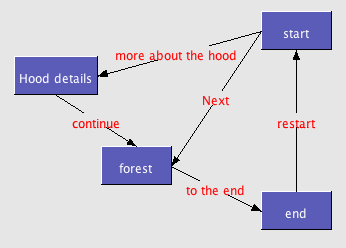
\includegraphics[width=6.5cm]{images/hypedyn-tutorial-1-figure-12}
  \caption{\textit{Setting up the ``Hood details'' node.}}
  \label{fig:tut1:setting_up_hood_details}
\end{figure} 

\subsection{Adding the condition}

Now we want to make it so that the reader can only follow the ``more about the
hood'' link if they've already read the ``end'' node. To do this, we need to
add a condition to the rule on the link between the ``start'' node and the
``Hood details'' node.

\begin{enumerate}
  \item Open the ``start'' text node, and select the link ``more about the
  hood''.
  \item Now click on the Edit link button. The Edit link dialogue will appear.
  \item Select the ``more about the hood'' rule, and click on the ``Edit Rule''
  button. The Edit rule dialogue will appear.

The Edit rule dialogue lets us create conditions which must be true for the
rule's actions to be performed. If there are multiple conditions, then you can
choose whether the actions will be performed when All or when Any of the
conditions are true, by using the Any/All pull-down menu. For now, leave this
pull-down menu at the default, All.

\item Click on the Add condition button. This will create a new condition which
must be satisfied for the actions to be performed, as shown in Figure
\ref{fig:tut1:adding_condition}.
 
\begin{figure}[ht]
  \centering
  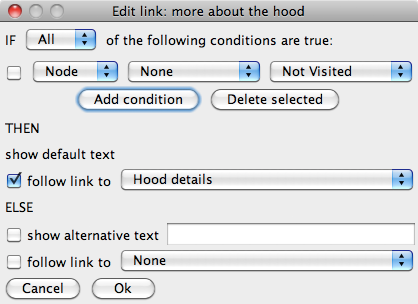
\includegraphics[width=7cm]{images/hypedyn-tutorial-1-figure-13}
  \caption{\textit{Adding a condition.}}
  \label{fig:tut1:adding_condition}
\end{figure} 

\item We want the action ``follow link to Hood details'' only to be performed if
the reader has gone through the entire story at least once. This means they have
to have visited the ``end'' node. Use the pull-down menus so that our condtion
reads ``Node end Visited''. (Your condition should look like Figure
\ref{fig:tut1:condition_hood_details}.) Then click Ok, and close the Edit link
dialogue.

\begin{figure}[ht]
  \centering
  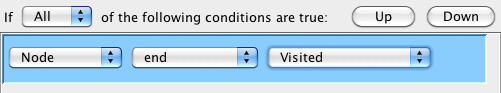
\includegraphics[width=8cm]{images/hypedyn-tutorial-1-figure-14}
  \caption{\textit{Condition for the ``Hood details''.}}
  \label{fig:tut1:condition_hood_details}
\end{figure} 

\item Close the ``start'' text node.
\end{enumerate}

\subsection{Testing the rule}

Now we will test out the rule.

\begin{enumerate}
  \item In the main window, click on the Run button.
  \item In the Reader you should see that the text ``red hood'' is bold,
  but not underlined. This indicates a link which cannot currently be
  followed, as shown in Figure \ref{fig:tut1:start_with_condition}.
 
\begin{figure}[ht]
  \centering
  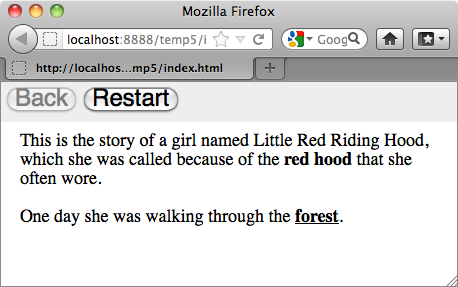
\includegraphics[width=9cm]{images/hypedyn-tutorial-1-figure-15}
  \caption{\textit{Start node with a link that cannot be followed.}}
  \label{fig:tut1:start_with_condition}
\end{figure} 

\item Now read through the story once, by clicking on ``forest'' in the
``start'' node, and then ``next'' in the ``forest'' node.
\item Finally, read back to the start by clicking on the ``back to start'' link
in the ``end'' node.
\item This time, you should see that the ``red hood'' text is a normal,
followable link. Click on the link to go to the ``Hood details'' node.

\item If you want to read the story again as if you've never read it, you need
to clear the Reader's history of which nodes have been visited.

In the Reader, click on the Restart. The Reader will go to the node which
we set as the start node, ``start'', and will clear its history.

\item You should now see that the ``red hood'' text is once again an
unfollowable link.
\end{enumerate}

We have now created a simple story, with links and conditions.

\section{Reading the story}

Once you have created and saved your story, you can export your story so that it
can be read by other people. Choose File->Export for web\ldots and specify the
name of the folder where you want to export your story. HypeDyn will create a
folder with that name, and save your story there as a web page. The folder
contains a number of supporting files, plus an ``index.html'' file. Keep all
these files together.

To read your exported story, open the ``index.html'' file in a web browser. This
is exactly the same as running the Reader from within the editor.

\section{Conclusion}

In this tutorial, we have created a simple hypertext fiction. Our story has a
main path, which tells a simplified version of the traditional folk tale
``Little Red Riding Hood''. Our story also has an alternative side path, which
gives the reader more information about Red's hood. This alternative side path
can only be read once the reader has visited the ``end'' node at the end of the
main story path. Although this is a simple story, it demonstrates all the
capabilities of HypeDyn, capabilities which are sufficient to create a more
complex hypertext fiction.

% \section{Final notes}

% As mentioned above, the HypeDyn hypertext editor is still a work-in-progress.
% Please let me know if you encounter any problems. Also, please post your
% questions about using the tool to the IVLE forum.

Please see tutorial 2 for more advanced features: links with multiple rules,
conditional text, and anywhere nodes.

\end{document}
